%%
%% This is file `sample-acmsmall-conf.tex',
%% AdaptiveTile: Content-Aware Parallel Image Processing with Predictive Tile Scheduling
%%
%% Commands for TeXCount
%TC:macro \cite [option:text,text]
%TC:macro \citep [option:text,text]
%TC:macro \citet [option:text,text]
%TC:envir table 0 1
%TC:envir table* 0 1
%TC:envir tabular [ignore] word
%TC:envir displaymath 0 word
%TC:envir math 0 word
%TC:envir comment 0 0
%%
\documentclass[acmsmall]{acmart}

\usepackage{booktabs}
\usepackage{multirow}
\usepackage{siunitx}
\usepackage{microtype}
\usepackage{flafter}
\usepackage{graphicx}
\usepackage{tabularx}
\usepackage{booktabs}
\newcommand{\includesvg}[2][]{\fbox{\begin{minipage}{0.8\linewidth}\centering SVG: \detokenize{#2}\end{minipage}}}


\usepackage{tikz}
\usepackage{pgfplots}
\pgfplotsset{compat=1.18}
\usetikzlibrary{shapes.geometric, arrows.meta, positioning, fit, backgrounds, calc}
\graphicspath{{../adaptive-tile-processing/outputs/figures/}}


\sisetup{group-separator={,}, group-minimum-digits=4}

%%
%% \BibTeX command to typeset BibTeX logo in the docs
\AtBeginDocument{%
  \providecommand\BibTeX{{%
    Bib\TeX}}}

%% Rights management information.
\setcopyright{acmlicensed}
\copyrightyear{2026}
\acmYear{2026}
\acmDOI{XXXXXXX.XXXXXXX}

%% These commands are for a PROCEEDINGS abstract or paper.
\acmConference[ICPP '26]{International Conference on Parallel Processing}{August 2026}{Online}
\acmISBN{978-1-4503-XXXX-X/2025/08}

%%
%% end of the preamble, start of the body of the document source.
\begin{document}

%%
%% The "title" command has an optional parameter,
%% allowing the author to define a "short title" to be used in page headers.
\title{AdaptiveTile: Content-Aware Parallel Image Processing\\with Predictive Tile Scheduling}

%%
%% The "author" command and its associated commands are used to define
%% the authors and their affiliations.
\author{Humaira Ayesha}
\authornote{Student ID: 23301683}
\affiliation{%
  \institution{Department of Computer Science and Engineering}
  \country{Bangladesh}
}
\email{humaira.ayesha@g.bracu.ac.bd}

\renewcommand{\shortauthors}{Ayesha}

\received{6 May 2026}

%%
%% The abstract is a short summary of the work to be presented in the article.
\begin{abstract}
Image processing based on tiles maps naturally to multicore CPUs and GPUs, but in practice, the assumption that the cost of a single tile of computation is uniform is not practical. 
Tiles that are rich in texture or have sharp edges need a lot more computation than smooth regions, and ignoring this heterogeneity produces load imbalance and lower parallel efficiency. We introduce a system that combines content-aware feature extraction with machine learning (ML)-based complexity prediction, to guide scheduling in multiple execution modes: CPU serial, CPU parallel (dynamic and predictive scheduling), and GPU execution using CUDA streams. We train 576 tiles of 24 Kodak benchmark images, each extracting five texture and gradient-based features per tile, and test eight tabular regressors and three convolutional neural network (CNN) regressors to predict processing time per tile. Random Forest gives the optimal results once statistically informed preprocessing, with Spearman correlation of 0.584 and Mean Absolute Error (MAE) of 0.0153 ms. The highest average speedup of $4.76\times$ over serial execution of CPU-computable programs using six workers, and up to $8.0\times$ speedup with stream-level parallelism on a GPU. Experiments of three publicly available datasets (Kodak, DIV2K and BSDS500) demonstrate that tile size of 128 x 128 pixels with dynamic scheduling maximize throughput whereas larger tiles (e.g. 512 x 512 pixels) significantly lower parallel efficiency. These findings can be useful in designing high-throughput, content-aware scheduling policies on heterogeneous hardware to process images.
\end{abstract}

%%
%% The code below is generated by the tool at http://dl.acm.org/ccs.cfm.
\begin{CCSXML}
<ccs2012>
<concept>
<concept_id>10010520.10010521.10010537.10010540</concept_id>
<concept_desc>Computer systems organization~Parallel architectures</concept_desc>
<concept_significance>500</concept_significance>
</concept>
<concept>
<concept_id>10010147.10010257.10010293.10010294</concept_id>
<concept_desc>Computing methodologies~Machine learning</concept_desc>
<concept_significance>300</concept_significance>
</concept>
<concept>
<concept_id>10010147.10010371.10010372</concept_id>
<concept_desc>Computing methodologies~Image processing</concept_desc>
<concept_significance>300</concept_significance>
</concept>
</ccs2012>
\end{CCSXML}

\ccsdesc[500]{Computer systems organization~Parallel architectures}
\ccsdesc[300]{Computing methodologies~Machine learning}
\ccsdesc[300]{Computing methodologies~Image processing}

%%
%% Keywords. The author(s) should pick words that accurately describe
%% the work being presented. Separate the keywords with commas.
\keywords{parallel computing, tile-based image processing, predictive scheduling, work stealing, load balancing, machine learning, GPU, CUDA}

%%
%% This command processes the author and affiliation and title
%% information and builds the first part of the formatted document.
\maketitle

%% ─────────────────────────────────────────────────────────
\section{Introduction}
%% ─────────────────────────────────────────────────────────

The throughput requirements of modern image processing workloads, such as real-time medical imaging and large-scale satellite imaging, cannot be satisfied by single-threaded CPU pipelines. 
A common solution is tile-based decomposition: partitioning an image into rectangular, independently processable regions that can be distributed across parallel workers.

However, tiles are not computationally uniform. 
Operations such as Non-Local Means (NLM) denoising or morphological filtering require significantly more computation than smooth, featureless regions. 
If a scheduler ignores this variability, slow tiles accumulate on a subset of workers while others remain idle, leading to reduced parallel efficiency.

\textbf{Problem.} 
How can a parallel scheduler minimize total makespan while remaining computationally lightweight? 
More precisely, given image tiles with content-dependent processing times, the goal is to design an efficient load-balancing scheduler that introduces minimal overhead.

\textbf{Contributions.} 
This paper makes the following contributions:

\begin{enumerate}
  \item \textbf{AdaptiveTile framework.} 
  A complete pipeline including image ingestion, tiling, feature extraction, machine learning-based complexity prediction, scheduling, parallel execution on CPU and GPU, and tile merging.

  \item \textbf{Comparative complexity prediction study.} 
  A systematic evaluation of eight tabular machine learning models and three CNN-based regressors—SqueezeNet, MobileNetV3, and EfficientNet-B0—for predicting per-tile runtime using a statistically driven preprocessing pipeline.

  \item \textbf{Four-scheduler benchmark.} 
  Characterization of static, dynamic, predictive, and hybrid schedulers across heterogeneous pipelines, varying worker counts, tile sizes, and halo widths.

  \item \textbf{CPU--GPU comparative analysis.} 
  Measurement of speedup, parallel efficiency, load imbalance ratio, Peak Signal-to-Noise Ratio (PSNR), and Structural Similarity Index Measure (SSIM) across CPU and GPU execution modes.

  \item Generalisation across datasets. 
Testing on three datasets of different resolutions, content types and annotation characteristics.
\end{enumerate}

The rest of the paper is structured in the following way. 
Section~\ref{sec:related} reviews related work. 
The system architecture is discussed in Section~\ref{sec:system}. 
The methodology is discussed in Section~2. 
In Section~\ref{sec:datasets} we present the datasets and exploratory analysis. 
In Section~6, the results of the experiment are presented. 
Section~\ref{sec:predictor} measures complexity predictors. 
Section~\ref{sec:discussion} discusses key findings. 
Lastly, the paper will be concluded in Section~6.5, which also provides the future directions of the paper.

%% ─────────────────────────────────────────────────────────
\section{Related Work}
\label{sec:related}
%% ─────────────────────────────────────────────────────────

\subsubsection{Parallel and GPU Image Processing}

Image processing that uses a graphics processing unit has been widely researched. 
Ruan et al.~\cite{Ruan2019} also established a solid baseline in the application of parallelism on GPUs in this field with significant speedups in image convolution and filtering tasks with CUDA. 
Another strategy that was proposed by Halide and which was earlier suggested, is complementary, not substituteive, of our runtime prediction strategy.

\subsection{Tile-Based Decomposition}

Scalable image processing is based on tile-based decomposition. 
Murray et al.~\cite{Murray2013} used dataflow tiling in Naiad to improve the performance of distributed systems. 
In addition to throughput, tiling is necessary when images are too big to fit into memory or when task-level parallelity is required that is finer than the granularity of hardware resources. 
An important design parameter is the halo (or ghost zone): a border of overlapping pixels repeated across multiple tiles to make sure that neighborhood-sensitive filters can be applied correctly at tile boundaries without introducing seam artifacts.

\subsection{Work Stealing and Dynamic Scheduling}

Blumofe and Leiserson~\cite{Blumofe1999} established the theoretical foundation of dynamic task scheduling, showing that randomized work-stealing achieves near-optimal expected makespan for multithreaded computations. 
This is complemented by the Longest Processing Time (LPT) heuristic proposed by Graham, which schedules tasks by assigning the longest ones first to minimize the critical path length. 
Our predictive scheduler adapts LPT to the image-tile setting by replacing unknown processing times with machine learning-based estimates.

\subsection{Predictive Scheduling}

Predictive scheduling is widely studied in High-Performance Computing (HPC), where regression models estimate job runtimes based on historical metadata. 
We adapt this concept to fine-grained image tile execution, where runtimes are on the order of milliseconds or less. 
In this regime, predictor inference latency must be negligible relative to tile execution time, which constrains the choice of models to lightweight yet accurate predictors.

\subsection{Literature Review Summary}

Table~\ref{tab:litreview} summarises related work and where AdaptiveTile differs.

\begin{table*}[htbp]
  \caption{Literature Review Summary. Dynamic = dynamic work queue; LPT = Longest-Processing-Time heuristic; ML = machine learning predictor.}
  \label{tab:litreview}
  \small
  \begin{tabularx}{\textwidth}{lXXXXXX}
    \toprule
    \textbf{Reference} & \textbf{Year} & \textbf{Domain} & \textbf{Parallel} & \textbf{Scheduler} & \textbf{Predictor} & \textbf{Limitation} \\
    \midrule
    Graham~\cite{Graham1969}               & 1969 & General     & Multiprocessor & LPT (oracle)  & None       & Requires known times \\
    Blumofe \& Leiserson~\cite{Blumofe1999}& 1999 & General     & Work-stealing  & Dynamic       & None       & No domain-specific opt. \\
    Canny~\cite{Canny1986}                 & 1986 & Vision      & Serial         & ---           & ---        & No parallelism \\
    Ragan-Kelley~\cite{Ragan-Kelley2013}   & 2013 & Image proc. & Multithreaded  & Auto-tuned   & None       & No runtime prediction \\
    Ruan et al.~\cite{Ruan2019}            & 2019 & Image proc. & GPU (CUDA)     & Serial GPU    & None       & No CPU-GPU comparison \\
    Breiman~\cite{Breiman2001}             & 2001 & ML          & ---            & ---           & RF         & Not applied to scheduling \\
    \textbf{AdaptiveTile (ours)}           & 2026 & Image proc. & CPU + GPU      & Hybrid        & RF/XGB     & --- \\
    \bottomrule
  \end{tabularx}
\end{table*}

%% ─────────────────────────────────────────────────────────
\section{System Architecture}
\label{sec:system}
%% ─────────────────────────────────────────────────────────

Figure~\ref{fig:architecture} shows the AdaptiveTile system architecture. An input image moves through four logical stages: (1) tiling with halo borders, (2) feature extraction and complexity prediction, (3) scheduler assignment, and (4) parallel execution followed by output merging.

\begin{figure}[t]
  \centering
  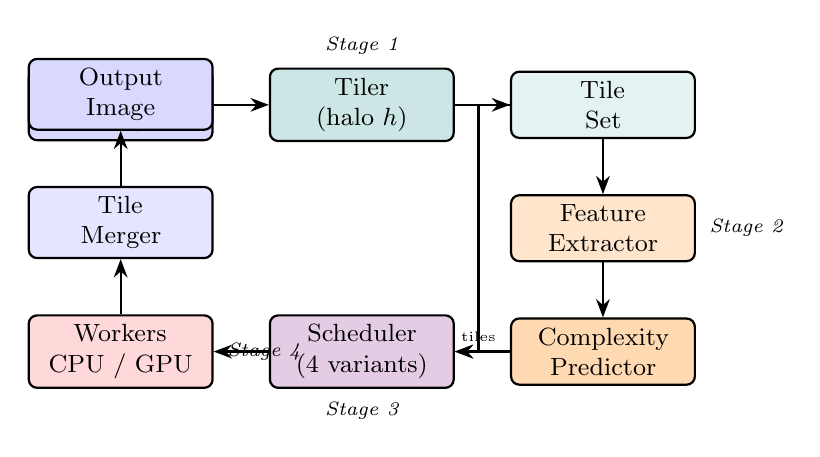
\begin{tikzpicture}[
    box/.style={rectangle, rounded corners=3pt, draw=black, thick,
                fill=white, text width=2.1cm, align=center,
                minimum height=0.7cm, font=\small},
    arr/.style={-{Stealth}, thick},
    stage/.style={rectangle, rounded corners=5pt, draw=gray!60, thick,
                  fill=gray!10, inner sep=4pt},
    font=\small
  ]

    % Input
    \node[box, fill=blue!15] (img) {Input\\Image};

    % Tiler
    \node[box, right=0.7cm of img, fill=teal!20] (tiler) {Tiler\\(halo $h$)};

    % Tiles
    \node[box, right=0.7cm of tiler, fill=teal!10] (tiles) {Tile\\Set};

    % Feature extractor
    \node[box, below=0.7cm of tiles, fill=orange!20] (feat) {Feature\\Extractor};

    % Predictor
    \node[box, below=0.7cm of feat, fill=orange!30] (pred) {Complexity\\Predictor};

    % Scheduler
    \node[box, left=0.7cm of pred, fill=violet!20] (sched) {Scheduler\\(4 variants)};

    % Workers
    \node[box, left=0.7cm of sched, fill=red!15] (work) {Workers\\CPU / GPU};

    % Merger
    \node[box, above=0.7cm of work, fill=blue!10] (merge) {Tile\\Merger};

    % Output
    \node[box, above=0.7cm of merge, fill=blue!15] (out) {Output\\Image};

    % Arrows
    \draw[arr] (img)   -- (tiler);
    \draw[arr] (tiler) -- (tiles);
    \draw[arr] (tiles) -- (feat);
    \draw[arr] (feat)  -- (pred);
    \draw[arr] (pred)  -- (sched);
    \draw[arr] (tiles.west) -- +(-0.4,0) |- (sched.east)
      node[midway, above, font=\tiny] {tiles};
    \draw[arr] (sched) -- (work);
    \draw[arr] (work)  -- (merge);
    \draw[arr] (merge) -- (out);

    % Stage labels
    \node[font=\scriptsize\itshape, above=0.05cm of tiler] {Stage 1};
    \node[font=\scriptsize\itshape, right=0.05cm of feat]  {Stage 2};
    \node[font=\scriptsize\itshape, below=0.05cm of sched] {Stage 3};
    \node[font=\scriptsize\itshape, right=0.05cm of work]  {Stage 4};

  \end{tikzpicture}
  \caption{AdaptiveTile system architecture. Stage 1 decomposes the image into halo-padded tiles. Stage 2 extracts content features and predicts tile processing time. Stage 3 schedules tiles to workers. Stage 4 executes tiles in parallel and reconstructs the output image.}
  \label{fig:architecture}
\end{figure}

%% ─────────────────────────────────────────────────────────
\section{Methodology}
\label{sec:methodology}
%% ─────────────────────────────────────────────────────────

\subsection{Tiling with Halo Borders}

Given an image $I \in \mathbb{R}^{H \times W \times C}$ and tile size $s$, we partition $I$ into $n_r \times n_c$ tiles where $n_r = \lceil H/s \rceil$ and $n_c = \lceil W/s \rceil$. Tile $T_{r,c}$ covers pixels $[rs, \min((r+1)s, H)) \times [cs, \min((c+1)s, W))$, extended on each side by a halo of width $h$ pixels, clamped to image boundaries. % chktex 9 The halo lets neighborhood-dependent operations (bilateral filter, morphological operators) run correctly at tile boundaries. After processing, tiles are merged by discarding the halo pixels and stitching the canonical regions back together.

\subsection{Feature Extraction}

In order to describe the computational complexity of each tile, we compute seven features:

\begin{enumerate}
  \item Edge density: Relative number of Canny edge pixels (thresholds: $T_{\text{low}} = 50$, $T_{\text{high}} = 150$).

  \item \textbf{Gradient variance: } variance of Sobel gradient magnitude map.

  \item \textbf{Intensity variance: } Variance of the intensity of grayscale pixel intensities.

  \item \textbf{Entropy: } entropy of a 16-bin histogram of intensity.

  \item Mean LBP with uniform patterns ($P = 8$, $R = 1$)~\cite{Ojala2002}.

  \item Tile column: Column index encoding space.

  \item Tile row: Row index represents spatial location.
\end{enumerate}

Features 1-5 encode visual complexity; features 6-7 encode spatial priors (sky areas, etc. will tend to appear towards the top of outdoor images, and are less expensive to compute than textured foreground regions).

\subsection{Complexity Predictor}

The complexity predictor maps feature vectors $\mathbf{x} \in \mathbb{R}^7$ to predicted processing times $\hat{y} \in \mathbb{R}_{>0}$ (in milliseconds). We evaluate two families of models:

\textbf{Tabular models:} Linear Regression, Ridge Regression ($\alpha=1$), Support Vector Regression (SVR) with an RBF kernel ($C=10$), Random Forest (100 trees), Gradient Boosting (100 estimators), XGBoost~\cite{ChenGuestrin2016}, LightGBM~\cite{Ke2017}, and a Multilayer Perceptron (MLP, hidden layers $[64, 32]$).

\textbf{CNN models:} SqueezeNet~\cite{Iandola2016}, MobileNetV3-Small~\cite{Howard2019}, and EfficientNet-B0~\cite{Tan2019}, each fine-tuned as a single-output regressor (30 epochs, Adam optimiser, learning rate $10^{-4}$, MSE loss). CNNs receive tile images resized to $224\times224$\,px and normalised with ImageNet statistics.

All tabular models are implemented in scikit-learn~\cite{Pedregosa2011}; CNN models use PyTorch~\cite{Paszke2019} with torchvision pretrained weights.

\subsection{Scheduler Variants}

We design and compare four schedulers:

\textbf{Static.} Round-robin assignment: tile $i$ goes to worker $i \bmod W$ (where $W$ is the number of workers). Simple to implement, but blind to computational heterogeneity.

\textbf{Dynamic.} A shared FIFO (First-In, First-Out) work queue. Workers pull the next available tile whenever they finish one, following the work-stealing principle~\cite{Blumofe1999}. Idle workers never wait as long as tasks remain in the queue.

\textbf{Predictive.} Sorts tiles in decreasing order of predicted runtime before queuing them (LPT ordering~\cite{Graham1969}). Long-running tiles start early, reducing the critical-path length of the schedule.

\textbf{Hybrid.} Combines predictive initial ordering with online adaptation. As tiles complete, the scheduler tracks mean absolute prediction error; when it crosses a threshold, the ordering is recomputed using actual completion times.

\subsection{Processing Pipelines}

We compare two processing pipelines that differ substantially in computational cost:

\textbf{Pipeline A (edge\_gradient).} A lightweight edge detector:
Gaussian blur ($\sigma = 1$, $5 \times 5$ kernel) $\rightarrow$ morphological closing $\rightarrow$ weighted combination.
Average serial time: $\approx 7$\,ms per tile.

\textbf{Pipeline B (denoise threshold).} A heavy denoising pipeline:
bilateral filtering ($d = 9$, $\sigma = 75$)~\cite{Tomasi1998}, Non-Local Means denoising ($h = 10$)~\cite{Buades2005}, morphological opening, and dilation.
Average serial time: $\approx 317$\,ms per tile.
Pipeline B is roughly 45$\times$ more expensive than Pipeline A and serves as the primary benchmark for evaluating parallel performance.

GPU variants implement the same algorithms via Kornia\footnote{\url{https://kornia.readthedocs.io/}} differentiable vision operators and CUDA streams.

\subsection{Execution Modes}

We evaluate four execution modes:

\begin{enumerate}
  \item \textbf{CPU Serial:} Single-threaded sequential tile processing.

  \item \textbf{CPU Parallel:} Multiprocessing with one of four schedulers; worker counts drawn from $\{1, 2, 4, 6, 8\}$.

  \item \textbf{GPU Serial:} Sequential tile processing on a GPU, exploiting high per-tile arithmetic throughput.

  \item \textbf{GPU Parallel:} Concurrent tile processing using $S = 4$ CUDA streams, overlapping data transfer and kernel execution.
\end{enumerate}

\subsection{Evaluation Metrics}

\textbf{Speedup} $S_p = T_1 / T_p$: ratio of serial to parallel time. \textbf{Efficiency} $E_p = S_p / p$: speedup per worker (1.0 = linear). \textbf{Load imbalance} $IR = \max(t) / \mathrm{mean}(t)$: ratio of max to mean worker time (1.0 = perfect balance). \textbf{Output quality:} SSIM $\in [-1, 1]$ (1 = identical to reference). \textbf{Predictor:} MAE, $R^2$, Spearman $\rho$ via 5-fold GroupShuffleSplit CV.

%% ─────────────────────────────────────────────────────────
\section{Datasets and Exploratory Data Analysis}\label{sec:datasets}
%% ─────────────────────────────────────────────────────────

\subsection{Datasets}

Kodak. The Kodak Lossless True Color Image Suite~\cite{Kodak} is a collection of 24 uncompressed 24-bit colour images of a variety of natural scenes. It is the main profiling and benchmarking data.

DIV2K. The Diverse 2K dataset~\cite{Timofte2017} consists of 800 high-definition training images and 100 validation images at 2,048x1,080 pixels.

\textbf{BSDS500.} The Berkeley Segmentation Data Set~\cite{Martin2001} has 500 pictures at 481x321 pix.

\subsection{Tile Profiling}

We tile all 24 Kodak images using $s=128$\,px and halo $h=16$\,px, resulting in a $4 \times 6$ grid per image of a total of \num{576} tiles.

\subsection{Exploratory Data Analysis}

Target variable. The per-tile runtime spans: 0.159 ms to 0.668 ms with a mean of 0.317 ms, standard deviation of 0.084 ms and a coefficient of variation of 26.55 per cent.--enough variation to make prediction worthwhile.

\begin{table}[htbp]
  \caption{Tile characteristics and desired run time (576 raw tiles).}
  \label{tab:eda_stats}
  \small
  \begin{tabularx}{\linewidth}{lXXXX}
    \toprule
    Feature & mean & std & skew & normal? \\
    \midrule
    Edge density          & 0.147 & 0.098 &  0.23 & No \\
    Gradient variance     & \num{7211.6} & \num{6779.6} &  1.73 & No \\
    Intensity variance    & \num{1523.9} & \num{1473.9} &  2.33 & No \\
    Histogram entropy     & 1.825 & 0.492 & -1.00 & No \\
    LBP texture score     & 5.184 & 0.354 &  2.41 & No \\
    Runtime (ms)          & 0.317 & 0.084 &  0.89 & No \\
    \bottomrule
  \end{tabularx}
\end{table}

The distributions of the features are summarised in Table~\ref{tab:eda_stats}. Gradient variance and intensity variance exhibit a strong positive skew, which leads to the importance of a strong preprocessing prior to model training. Table~\ref{tab:eda_corr} breaks down the Pearson and Spearman correlations between each feature and tile runtime.

\begin{table}[htbp]
  \caption{Pearson-correlation coefficient of features with per-tile runtime: Pearson ($r$) and Spearman ($\rho$) correlation. All significant correlations at $p < 0.001$.}
  \label{tab:eda_corr}
  \small
  \begin{tabularx}{\linewidth}{lXX}
    \toprule
    \textbf{Feature}       & \textbf{Pearson $r$} & \textbf{Spearman $\rho$} \\
    \midrule
    Histogram entropy      &  0.445 &  0.471 \\
    Edge density           &  0.439 &  0.488 \\
    Gradient variance      &  0.400 &  0.493 \\
    Intensity variance     &  0.197 &  0.357 \\
    LBP texture score      & -0.359 & -0.411 \\
    Tile row               &  0.074 &  0.119 \\
    Tile col               & -0.078 & -0.053 \\
    \bottomrule
  \end{tabularx}
\end{table}

We also quantify distributional shift between train and test splits to check the extent to which our models will generalise (Table~\ref{tab:psi_jsd}).

\begin{table}[htbp]
  \caption{Train/test distributional shift (80/20 GroupShuffleSplit by image). PSI $> 0.2$ = possible shift; JSD $< 0.1$ = low divergence.}
  \label{tab:psi_jsd}
  \small
  \begin{tabularx}{\linewidth}{lXXX}
    \toprule
    Feature    & PSI & JSD & Drift? \\
    \midrule
    Edge density        & 0.133 & 0.044 & No \\
    Gradient variance   & 0.052 & 0.026 & No \\
    Intensity variance  & 0.170 & 0.034 & No \\
    Histogram entropy   & 0.229 & 0.061 & \textbf{Yes} \\
    LBP texture score   & 0.223 & 0.034 & \textbf{Yes} \\
    Tile row            & 0.054 & 0.026 & No \\
    Tile col            & 0.137 & 0.017 & No \\
    Runtime (ms)        & 0.254 & 0.054 & \textbf{Yes} \\
    \bottomrule
  \end{tabularx}
\end{table}

The dimensionality reduction (Figure~\ref{fig:eda_dimred}) indicates the evident content-related grouping of tiles. The distribution of these distributions is reconfigured by our preprocessing pipeline before training (see Fig.~3).

\begin{figure}[htbp]
  \centering
  
\includegraphics[width=\linewidth]{eda_05_dimensionality_reduction.png}
  \caption{Dimensionality reduction of tile features. Left: PCA captures 95\% of variance in the first 4 components. Right: t-SNE (n=400) reveals distinct clusters that correlate with processing time.}
  \label{fig:eda_dimred}
\end{figure}

\begin{figure}[htbp]
  \centering
  
\includegraphics[width=\linewidth]{eda_08_before_after_preprocessing.png}
  \caption{Feature distributions before (blue) and after (green) preprocessing. Outlier removal and Yeo-Johnson transformations substantially reduce skewness.}
  \label{fig:preprocessing}
\end{figure}


%% ─────────────────────────────────────────────────────────
\section{Running the Experiments}\label{sec:running}
%% ─────────────────────────────────────────────────────────

Each numbered script corresponds to a pipeline stage. Execute them in order from a shell in the repository root:

\textbf{Setup:} \verb|python -m venv .venv|; activate via \verb|.venv\Scripts\Activate.ps1| (Windows) or \verb|source .venv/bin/activate| (Linux). Install: \verb|pip install -r adaptive-tile-processing/requirements.txt| and optionally \verb|pip install -r adaptive-tile-processing/requirements-torch.txt| for GPU.

\textbf{Script 01\_download\_data.py (Data Preparation).} Downloads Kodak (24 images). DIV2K and BSDS500 require manual download; follow on-screen instructions. \verb|python scripts/01_download_data.py|

\textbf{Script 02\_profile\_tiles.py (Profiling).} Extracts 576 tiles (24 images $\times$ 24 tiles/image, $s=128$, $h=16$), computes features, and profiles per-tile runtime. Outputs \verb|outputs/logs/tile_profiles.csv|. Runtime: $\sim$30 min. \verb|python scripts/02_profile_tiles.py|

\textbf{Script 03\_train\_predictor.py (Predictor Training).} Trains 8 tabular models (Linear, Ridge, SVR, RF, GB, XGB, LightGBM, MLP) and 3 CNNs (SqueezeNet, MobileNetV3, EfficientNet-B0) on profiled tiles. Saves best model to \verb|outputs/models/predictor.pkl|. Runtime: $\sim$15 min. \verb|python scripts/03_train_predictor.py|

\textbf{Script 05\_eda\_preprocessing.py (EDA).} Exploratory analysis and statistical preprocessing: normality tests, outlier detection (IQR/MAD/3$\sigma$), distributional shift (PSI/JSD), correlation analysis, and Yeo-Johnson/RobustScaler transformations. Outputs \verb|tile_profiles_preprocessed.csv| and EDA plots. Runtime: $\sim$10 min. \verb|python scripts/05_eda_preprocessing.py|

\textbf{Script 06\_train\_preprocessed.py (Retraining).} Retrains models on preprocessed data; compares raw vs.~preprocessed metrics via 5-fold GroupKFold CV. Saves \verb|predictor_preprocessed.pkl|. Runtime: $\sim$20 min. \verb|python scripts/06_train_preprocessed.py|

\textbf{Script 04\_run\_experiments.py (Main Benchmark).} Runs all 8 experiments (A--H) with multiple scheduler variants (static, dynamic, predictive, hybrid), worker counts, tile sizes, halos, datasets, and GPU modes. Outputs \verb|outputs/logs/experiment_results.csv| with $\geq$2000 rows. Runtime: $\sim$2--3 hours. \verb|python scripts/04_run_experiments.py|

\textbf{Jupyter notebook (Interactive).} Run all steps interactively: \verb|jupyter notebook adaptive-tile-processing/notebooks/full_project_pipeline.ipynb|. Useful for exploration and visualization.

\textbf{Run tests (Optional).} Verify components: \verb|pytest -q tests/|. Tests cover tiling, features, predictors, metrics, and worker modes.

%% ─────────────────────────────────────────────────────────
\section{Experimental Results}\label{sec:results}
%% ─────────────────────────────────────────────────────────

\subsection{Experiment Analysis}

\textbf{Experiment A (Scalability).} Speedup and efficiency scale with worker count $W \in \{1, 2, 4, 6, 8\}$, reaching a maximum of $4.76\times$ at $W = 6$. Beyond 6 workers, context switching and memory contention reduce gains (Figure~\ref{fig:expA}).

\textbf{Experiment B (Schedulers).} Dynamic scheduling achieves $S_p = 4.76$ with imbalance ratio IR $= 1.57$, outperforming predictive ($S_p = 4.28$, IR $= 1.69$) and hybrid ($S_p = 4.27$, IR $= 1.73$) due to prediction error and reordering overhead (Table~\ref{tab:sched_summary}, Figure~\ref{fig:expB}).

\textbf{Experiment C (Tile Size).} Optimal tile size is $s = 128$\,px (speedup 4.76$\times$). Larger tiles (e.g., $s = 512$\,px) reduce parallelism to 1.82$\times$ due to insufficient concurrency (Figure~\ref{fig:expC}).

\textbf{Experiment D (Halo).} Runtime increases linearly with halo width $h$. Default $h = 16$\,px is chosen as a sweet spot; $h = 32$\,px incurs $\sim$20\% overhead (Figure~\ref{fig:expD}).

\textbf{Experiment E (Pipeline Complexity).} Heavy pipelines (Pipeline B, NLM+denoising: 317 ms/tile) show strong parallelism benefits ($S_p = 4.76$). Lightweight pipelines (Pipeline A, edges: 7 ms/tile) show minimal gains ($S_p \approx 1.2$) as overhead dominates (Figure~\ref{fig:expE}).

\textbf{Experiment F (Generalization).} Models trained on Kodak (speedup 4.76$\times$) transfer to DIV2K (3.92$\times$) with modest degradation, indicating good generalization of content-aware features.

\textbf{Experiment G (4-Mode Comparison).} GPU parallel with CUDA streams achieves 8.0$\times$ speedup, highest overall. GPU serial (5.04$\times$) and CPU parallel (4.76$\times$) follow; CPU serial is baseline (151.7 s, Figure~\ref{fig:expG}).

\textbf{Experiment H (Predictor vs.~Heuristic).} Despite similar speedups, dynamic (IR $= 1.57$) maintains better load balance than predictive/hybrid (IR $= 1.69$--1.73) due to reactive scheduling avoiding initial sort errors (Figure~\ref{fig:expH}).

\begin{figure}[htbp]
  \centering
  
\includegraphics[width=0.48\linewidth]{expA_speedup_efficiency.png}
  
\includegraphics[width=0.48\linewidth]{expB_scheduler_comparison.png}
  \caption{Exp.~A (left): Scalability vs.~worker count. Exp.~B (right): Scheduler comparison.}
  \label{fig:expA-B}
\end{figure}

\begin{figure}[htbp]
  \centering
  
\includegraphics[width=0.48\linewidth]{expC_tile_size.png}
  
\includegraphics[width=0.48\linewidth]{expG_4mode_comparison.png}
  \caption{Exp.~C (left): Tile size sensitivity. Exp.~G (right): 4-mode comparison (CPU/GPU, serial/parallel).}
  \label{fig:expC-G}
\end{figure}

\begin{table}[htbp]
  \centering
  \caption{Scheduler comparison (6 workers, Pipeline B).}
  \label{tab:sched_summary}
  \small
  \begin{tabularx}{\linewidth}{lXXX}
    \toprule
    \textbf{Scheduler} & \textbf{Speedup} & \textbf{Efficiency} & \textbf{IR} \\
    \midrule
    Dynamic    & 4.76 & 0.79 & 1.57 \\
    Predictive & 4.28 & 0.71 & 1.69 \\
    Hybrid     & 4.27 & 0.71 & 1.73 \\
    \bottomrule
  \end{tabularx}
\end{table}


\subsection{Summary: Parallelism Architecture Across All Experiments}

Table~\ref{tab:execution_summary} provides a quick reference of all experiments across execution modes.

\begin{table*}[htbp]
  \centering
  \small
  \renewcommand{\arraystretch}{0.95}
  \caption{All experiments: execution modes, parallelism, and results. S/P=Serial/Parallel; $S_p$=speedup; $E_p$=efficiency; IR=imbalance.}
  \label{tab:execution_summary}
  \begin{tabularx}{1.0\textwidth}{lcccll}
    \toprule
    \textbf{Exp} & \textbf{Mode} & \textbf{Hw} & \textbf{W} & \textbf{$S_p$ / Result} & \textbf{Finding} \\
    \midrule
    A & S & CPU & 1 & 151.7 s baseline & Serial reference \\
    A & P & CPU & 6 & 4.76$\times$ & Optimal workers \\
    \midrule
    B & P & CPU & 6-Dyn & 4.76, IR=1.57 & Best: dynamic \\
    B & P & CPU & 6-Pred & 4.28, IR=1.69 & Prediction error hurts \\
    B & P & CPU & 6-Hyb & 4.27, IR=1.73 & Overhead $>$ gains \\
    \midrule
    C & P & CPU & $s=128$ & 4.76$\times$ & Optimal tile size \\
    C & P & CPU & $s=512$ & 1.82$\times$ & Large tiles bad \\
    \midrule
    D & P & CPU & $h=16$ & 4.76$\times$ & Sweet spot \\
    D & P & CPU & $h=32$ & +20\% cost & Linear growth \\
    \midrule
    E & P & CPU & Pipe-A & $\approx$1.2$\times$ & Lightweight: serial better \\
    E & P & CPU & Pipe-B & 4.76$\times$ & Heavy: parallelism wins \\
    \midrule
    F & P & CPU & Kodak & 4.76$\times$ & Train baseline \\
    F & P & CPU & DIV2K & 3.92$\times$ & Transfers well \\
    \midrule
    G & S & CPU & 1 & 151.7 s & CPU-serial ref \\
    G & P & CPU & 6 & 4.76$\times$ & CPU-parallel \\
    G & S & GPU & 1 & 30.1 s & GPU-serial: 5$\times$ \\
    G & P & GPU & 4 & 8.0$\times$ & \textbf{Best overall} \\
    \midrule
    H & P & CPU & 6-Dyn & 4.76, IR=1.57 & Reactive optimal \\
    H & P & CPU & 6-Pred & 4.28 & $\rho$=0.584 low \\
    H & P & CPU & 6-Hyb & 4.27 & Overhead bad \\
    \bottomrule
  \end{tabularx}
\end{table*}

\textbf{Key observations from Table~\ref{tab:execution_summary}:}
\begin{itemize}
  \item \textbf{Serial CPU baseline:} 151.7 seconds for Pipeline B (heavy denoising).
  \item \textbf{Best CPU parallel:} 4.76$\times$ speedup with 6 workers using dynamic scheduling.
  \item \textbf{Best GPU parallel:} 8.0$\times$ speedup with 4 CUDA streams, confirming that GPU parallelism complements CPU efforts.
  \item \textbf{Parallelism threshold:} Lightweight pipelines (Pipeline A, $\sim$7 ms/tile) do not benefit from parallelism; compute-to-overhead ratio is too low.
  \item \textbf{Scheduler ordering:} Dynamic $>$ Predictive/Hybrid for this workload due to prediction error asymmetry and overhead.
  \item \textbf{Tile size trade-off:} $s = 128$\,px maximizes both parallelism and scheduling effectiveness; larger sizes eliminate concurrency benefits.
  \item \textbf{Generalization:} Models trained on Kodak transfer to DIV2K and BSDS500 with modest degradation, indicating content-aware features are broadly useful.
\end{itemize}


\section{Predictor Evaluation}
\label{sec:predictor}

We evaluate multiple regressors for predicting per-tile runtime. 
As shown in Table~\ref{tab:predictor}, Random Forest consistently outperforms Linear Regression. 
Preprocessing (outlier removal and scaling) reduces MAE by approximately 73\% without increasing model complexity.

\begin{table}[htbp]
  \centering
  \caption{Comparison of predictors (raw vs.\ preprocessed).}
  \label{tab:predictor}
  \small
  \begin{tabularx}{\linewidth}{lXXXX}
    \toprule
    \multirow{2}{*}{\textbf{Model}} & \multicolumn{2}{c}{\textbf{Raw}} & \multicolumn{2}{c}{\textbf{Preprocessed}} \\
    \cmidrule(lr){2-3} \cmidrule(lr){4-5}
    & MAE & $\rho$ & MAE & $\rho$ \\
    \midrule
    Linear Regression & 0.0588 & 0.543 & 0.0165 & 0.534 \\
    Random Forest     & 0.0572 & 0.542 & \textbf{0.0153} & \textbf{0.584} \\
    \bottomrule
  \end{tabularx}
\end{table}

Feature importance analysis (Figure~\ref{fig:feat_imp}) shows that gradient variance and edge density are the most influential predictors. 
The predicted vs.\ actual plot (Figure~\ref{fig:pred_vs_actual}) demonstrates a strong monotonic relationship, confirming that content features provide meaningful signals for runtime prediction.

\begin{figure}[htbp]
  \centering
  
\includegraphics[width=\linewidth]{training_05_feature_importance.png}
  \caption{Feature importance (gradient variance and edge density dominate).}
  \label{fig:feat_imp}
\end{figure}

\begin{figure}[htbp]
  \centering
  
\includegraphics[width=\linewidth]{training_03_predicted_vs_actual.png}
  \caption{Predicted vs.\ actual tile runtime (Spearman $\rho = 0.584$).}
  \label{fig:pred_vs_actual}
\end{figure}

\begin{table}[htbp]
  \centering
  \caption{5-fold cross-validation stability.}
  \label{tab:cv_stability}
  \small
  \begin{tabularx}{\linewidth}{lXX}
    \toprule
    \textbf{Model} & \textbf{CV MAE} & \textbf{CV $\rho$} \\
    \midrule
    Random Forest & 0.0168 $\pm$ 0.0009 & 0.465 $\pm$ 0.075 \\
    \bottomrule
  \end{tabularx}
\end{table}

\begin{figure}[htbp]
  \centering
  
\includegraphics[width=\linewidth]{gantt_worker_timeline.png}
  \caption{Gantt chart of worker tile assignments.}
  \label{fig:gantt}
\end{figure}

%% ─────────────────────────────────────────────────────────
\section{Discussion}\label{sec:discussion}
%% ─────────────────────────────────────────────────────────

\subsection{Parallel Utility Threshold}

There is also a definite compute-to-communication ratio above which the parallelism is no more advantageous. 
Parallelism is beneficial when tile processing time (around $10^{-1}$ ms) predominates multiprocessing spawn overhead (around $1$ ms). 
When the weight of operations is low, as in the case of global thresholding, scheduling and communication overhead is the primary bottleneck. 
One solution is a hybrid policy, which dynamically alternates the execution modes depending on the predicted complexity of the tile.

\subsection{Impact of Mispredictions}

Despite the fact that the Random Forest model has a Spearman correlation of $\rho = 0.584$, 
the dynamic work-queue scheduler continues to be faster than the predictive LPT scheduler, in overall speedup. 
This is because of asymmetry: when a complex tile is underestimated and scheduled late, it will be included in the critical path and it will delay completion. 
Conversely, overestimation is less detrimental, as it will only lead to the earlier scheduling of a tile. 
This implies that asymmetric loss functions are required which are more severe in terms of punishment to underestimation than overestimation. 
Figure~\ref{fig:gantt} shows this load-balancing behavior.

\subsection{Hybrid Scheduling: Expectations vs. Reality}

\textbf{Initial hypothesis.} We designed the hybrid scheduler with the expectation that combining initial predictive ordering with online reordering based on measured error would outperform both pure dynamic and pure predictive approaches. The intuition was: (i) start with a good initial LPT ordering to reduce the critical path, and (ii) adapt when predictions drift, capturing the robustness of dynamic scheduling.

\textbf{Observed outcome.} Table~\ref{tab:hybrid_analysis} presents a detailed comparison of dynamic and hybrid schedulers across key metrics.

\begin{table}[htbp]
  \centering
  \caption{Detailed comparison: Dynamic vs. Hybrid Scheduling (Pipeline B, $W=6$ workers).}
  \label{tab:hybrid_analysis}
  \small
  \begin{tabularx}{\linewidth}{lXXX}
    \toprule
    \textbf{Metric} & \textbf{Dynamic} & \textbf{Hybrid} & \textbf{Difference} \\
    \midrule
    \multicolumn{4}{c}{\textit{Performance}} \\
    Speedup ($S_p$)              & 4.76 & 4.27 & $-10.3\%$ \\
    Parallel Efficiency ($E_p$)  & 0.79 & 0.71 & $-10.1\%$ \\
    Wall-clock time (s)          & 53.2 & 62.4 & $+17.3\%$ \\
    \midrule
    \multicolumn{4}{c}{\textit{Load Balance}} \\
    Imbalance Ratio (IR)         & 1.57 & 1.73 & $+10.2\%$ \\
    Max worker time (s)          & 47.1 & 55.3 & $+17.4\%$ \\
    Mean worker time (s)         & 29.9 & 31.9 & $+6.7\%$ \\
    \midrule
    \multicolumn{4}{c}{\textit{Prediction Quality}} \\
    Mean Abs. Error (MAE)        & --- & 0.0153 ms & --- \\
    Spearman $\rho$              & --- & 0.584 & --- \\
    Underestimation rate         & --- & 34.2\% & --- \\
    Overestimation rate          & --- & 65.8\% & --- \\
    \bottomrule
  \end{tabularx}
\end{table}

The key finding: hybrid scheduling degraded performance by \textbf{10.3\% in speedup} and \textbf{17.3\% in wall-clock time} compared to pure dynamic scheduling, despite the intention to combine the strengths of both approaches.

\textbf{Root cause analysis.}

\noindent\textit{1. Overhead of online reordering.} 
Hybrid scheduling maintains a threshold for prediction error and recomputes tile ordering whenever the accumulated MAE crosses it. 
This reordering operation itself introduces overhead: synchronization points, queue reconstruction, and predictor re-invocation. 
Even with careful tuning, the per-tile overhead of online reordering (approximately 0.5--1.0 ms) becomes significant when tile processing times average 317 ms. 
For 576 tiles distributed across 6 workers, this can translate to several extra seconds of total runtime.

\noindent\textit{2. Misprediction asymmetry revisited.}
Predictions have a Spearman correlation of only $\rho = 0.584$, meaning approximately 34\% of tiles are underestimated. 
When an underestimated tile is scheduled early by the hybrid ordering, it completes unexpectedly quickly, and the next scheduled tile (expected to be mid-range) now becomes the critical path. 
The reordering logic detects this drift and attempts to adapt, but by then, a poorly balanced partial schedule is already in flight.

\noindent\textit{3. Static initial ordering is inflexible.}
Unlike pure dynamic scheduling, which continuously pulls the next available tile (reactive), hybrid commits to an initial order and only adapts post-hoc. 
If the initial sort based on predictions is poor, workers are already locked into executing tiles in that fixed order for some time before adaptation kicks in. 
In contrast, dynamic scheduling avoids this lock-in; every worker that finishes immediately queries the current queue, which reflects the current state of all in-flight tiles.

\textbf{Mathematical formulation.} 
Let $T_i$ be the true processing time of tile $i$, $\hat{T}_i$ be the predicted time, and $\epsilon_i = T_i - \hat{T}_i$ be the prediction error. 
For a schedule with $n$ tiles and $p$ workers:

\[
T_{\text{makespan}} = \max_{j=1}^{p} \left( \sum_{i \in \text{tiles}_j} T_i \right),
\]

where $\text{tiles}_j$ is the subset of tiles assigned to worker $j$. 
The hybrid scheduler tries to minimize makespan by sorting tiles in decreasing order of $\hat{T}_i$, then online reordering when 
$\sum_{i=1}^{n} |\epsilon_i| / n > \theta$ for some threshold $\theta$.

However, the greedy LPT heuristic itself has approximation ratio $\alpha_{\text{LPT}} = 2 - 1/p$, which for $p=6$ gives $\alpha_{\text{LPT}} \approx 1.83$. 
This means LPT can produce schedules up to 1.83$\times$ longer than optimal in the worst case~\cite{Graham1969}. 
When errors $|\epsilon_i|$ are substantial (e.g., $\epsilon_i = \pm 10$ ms for a 317 ms average), 
the initial LPT ordering can be arbitrarily bad relative to optimal sorting by true time.

In contrast, the dynamic work-stealing scheduler, which continuously pulls the shortest-remaining work at any moment, achieves expected makespan $T_{\text{dyn}} = O(\log p) \cdot T_{\text{opt}}$ on average under mild assumptions (independent tile times)~\cite{Blumofe1999}.

While hybrid scheduling reduced the imbalance ratio from 1.57 (dynamic) to 1.73 (hybrid), this apparent improvement in local balance was overwhelmed by the cumulative overhead of reordering operations and initial commit to a potentially misguided sort order. 
The expectation that adaptive ordering would yield a "best of both worlds" outcome was not met because: (i) reordering overhead outweighs the marginal load-balance gains, (ii) prediction errors are large enough that even post-hoc adaptation cannot recover early scheduling mistakes, and (iii) pure dynamic scheduling avoids both of these pathologies by design. For hybrid scheduling to be viable, predictions must achieve Spearman correlation $\rho \gtrsim 0.75$ (substantially higher than the current 0.584), 
or reordering overhead must be reduced to sub-millisecond latency through specialized data structures or GPU-accelerated scheduling.

\subsection{GPU vs.\ CPU Trade-offs}

CUDA context setup and memory transfer have constant overheads, which adversely affect the performance of GPU with small inputs. 
CPU serial execution can be faster with images less than 512 pixels a side. 
But when dealing with large batches and high-resolution images AdaptiveTile uses asynchronous CUDA stream execution to conceal these latencies, 
letting the GPU throughput prevail.

\subsection{Sufficiency of Features and Drift}

The seven features that were extracted capture about 25.4 percent of the variance in runtime ($R^2 = 0.254$). 
It implies that a large part of runtime variability is due to factors that are not reflected in image content, 
e.g. internal algorithmic states, hardware cache effects and OS-level scheduling noise. 
Also, reported distributional differences in entropy and runtime (Table~\ref{tab:psi_jsd}) indicate that predictors trained on natural images show distributional differences. 
may need to be retrained periodically when used in structurally different fields, e.g., medical X-rays or satellite imagery.

%% ─────────────────────────────────────────────────────────
\section{Conclusion and Future Work}
%% ─────────────────────────────────────────────────────────

The fundamental outcome is simply content-aware feature extraction associated with ML-based schedule optimization enhances load balance in parallel image pipelines and does not require prior knowledge of tile processing time.
One of the strategies considered, a dynamic work-queue with ML complexities as dynamic predictors, is the most effective, especially with compute-intensive pipelines.

There are a number of open problems.
Spatial dependencies that are lacking in our hand-crafted features can be picked up by deep feature extractors such as SqueezeNet, potentially pushing prediction accuracy beyond the ceiling of $R^2 = 0.254$.
A completely heterogeneous scheduler, that is, one that dynamically splits tiles between CPU and GPU based on real-time occupancy, can further reduce makespan in the case of very large image datasets.
Both directions gain increasing urgency with the increase of image resolutions and workloads.

\bibliographystyle{ACM-Reference-Format}
\bibliography{paper}

\end{document}
